\documentclass[10pt,journal,compsoc]{IEEEtran}

\usepackage[pdftex]{graphicx}    
\usepackage{cite}
\hyphenation{op-tical net-works semi-conduc-tor}


\begin{document}

\title{Robotic Inference Application on Flower Recognition using GoogLeNet}

\author{Peng Xu}

\markboth{Inference project, Robotic Nanodegree, Udacity}%
{}
\IEEEtitleabstractindextext{%

\begin{abstract}
The project is an attempt to practice deep learning on Nvidia DIGITS and prepare for robotic inference applications. A supplied dataset is given as a benchmark to test the pipeline of training and evaluating a model. The GoogLeNet network is applied and has achieved 75\% accuracy and 10 ms inference speed which satisfied the project requirements.
\end{abstract}

% Note that keywords are not normally used for peerreview papers.
\begin{IEEEkeywords}
Robotic Inference, Deep Learning, Image Classification.
\end{IEEEkeywords}}


\maketitle
\IEEEdisplaynontitleabstractindextext
\IEEEpeerreviewmaketitle
\section{Introduction}
\label{sec:introduction}

\IEEEPARstart{T}{he} project aims to apply deep learning methods on robotic inference applications. Imagine there is a garden where several kinds of flowers are planted. The task for the robot is to recognize the flower species. Deep Learning is used to have an end-to-end learning and a state-of-art deep convolutional network model, GoogLeNet is used to train this model.

The training and evaluation process could be greatly simplified by Nvidia DIGITS platform. With only filling the hyperparameters, the data preprocessing and model building could be done using Cloud Computing.

Hopefully, the trained model could be directly applied on a Jetson TX1/TX2.
 
\section{Background}

Deep learning has absolutely dominated computer vision over the last few years, achieving top scores on many tasks and their related competitions. The most popular and well known of these computer vision competitions is ImageNet \cite{imagenet_cvpr09}. The ImageNet competition tasks researchers with creating a model that most accurately classifies the given images in the dataset.

Over the past few years, deep learning techniques have enabled rapid progress in this competition, even surpassing human performance.

\begin{figure}[thpb]
      \centering
      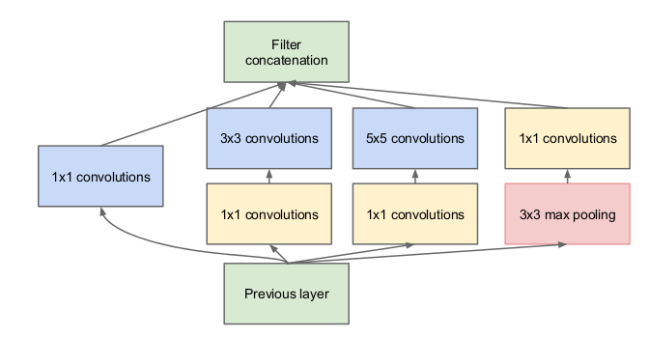
\includegraphics[width=\linewidth]{images/googlenet.png}
      \caption{Inception Module from GoogLeNet.}
      \label{fig:googlenet}
\end{figure}

The GoogLeNet \cite{googlenet} architecture was the first to really address the issue of computational resources along with multi-scale processing in the paper “Going Deeper with Convolutions”. As we keep making our classification networks deeper and deeper, we get to a point where we’re using up a lot of memory. Additionally, different computational filter sizes have been proposed in the past: from 1x1 to 11x11; how do you decide which one? The inception module and GoogLeNet tackles all of these problems with the following contributions:

Through the use of 1x1 convolutions before each 3x3 and 5x5, the inception module reduces the number of feature maps passed through each layer, thus reducing computations and memory consumption!

The inception module has 1x1, 3x3, and 5x5 convolutions all in parallel. The idea behind this was to let the network decide, through training what information would be learned and used. It also allows for multi-scale processing: the model can recover both local features via smaller convolutions and high abstracted features with larger convolutions. 

GoogLeNet was one of the first models that introduced the idea that CNN layers didn’t always have to be stacked up sequentially. The authors of the paper showed that you can also increase network width for better performance and not just depth.

\section{Data Acquisition}

\subsection{Supplied Dataset}

Supplied Data from Udacity was having 3 classes (Bottle, Candy Box, Nothing).

\begin{table}[h]
\caption{Supplied Data}
\label{table_example}
\begin{center}
\begin{tabular}{|c|c|c|}
\hline
Bottle & 3426 &	256x256x3\\
\hline
Candy Box &	1871 & 256x256x3\\
\hline
Nothing & 2273 & 256x256x3\\
\hline
Total & 7570 & \\
\hline
\end{tabular}
\end{center}
\end{table}

In Fig. \ref{fig:supplied-examples} some example images are shown as examples picked from the supplied dataset.

\begin{figure}
    \centering
    \begin{tabular}{cc}
    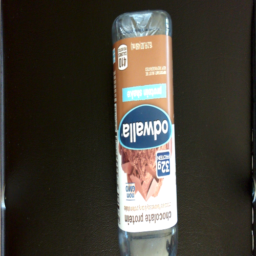
\includegraphics[width=35mm]{images/example-bottle.png} &
    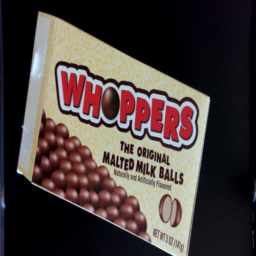
\includegraphics[width=35mm]{images/example-candy-box.png} \\
    (a) Bottle & (b) Candy Box \\[6pt]
    \hspace{0mm}
    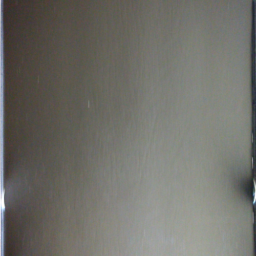
\includegraphics[width=35mm]{images/example-nothing.png} \\
    (c) Nothing \\[6pt]
    \end{tabular}
    \caption{Example data in Supplied dataset.}
    \label{fig:supplied-examples}
\end{figure}

\subsection{Collected Dataset}

The dataset, Flowers, contains 4242 images of flowers. The data collection is based on the data flicr, google images, yandex images. The datastet to recognize 5 classes of flowers:: chamomile, tulip, rose, sunflower, dandelion. For each class there are about 800 Images. Images are not high resolution, about 320x240 pixels. Images are not reduced to a single size, they have different proportions.

In Fig. \ref{fig:flowers-examples} some example images are shown as examples picked from the collected dataset.

%example image in the dataset
\begin{figure}
    \centering
    \begin{tabular}{cc}
    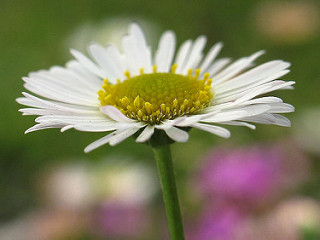
\includegraphics[width=35mm]{images/example-daisy.jpg} &
    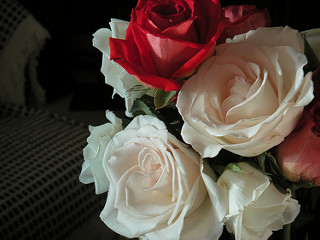
\includegraphics[width=35mm]{images/example-rose.jpg} \\
    (a) Daisy & (b) Rose \\[6pt]
    \hspace{0mm}
    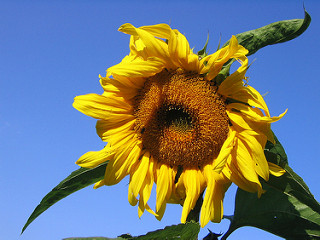
\includegraphics[width=35mm]{images/example-sun-flower.jpg} & 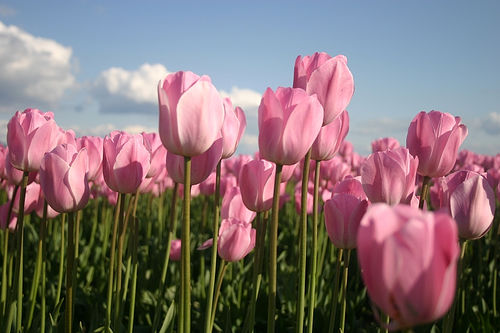
\includegraphics[width=35mm]{images/example-tulip.jpg} \\
    (c) Sun-Flower & (d) Tulip \\[6pt]
    \end{tabular}
    \caption{Example data in Collected dataset.}
    \label{fig:flowers-examples}
\end{figure}

\section{Results}

\subsection{On Supplied Dataset}

GoogLeNet trained on the supplied dataset converged quickly within 5 epochs. The training accuracy and validation accuracy were almost the same and around 100\%.

\begin{figure}[thpb]
      \centering
      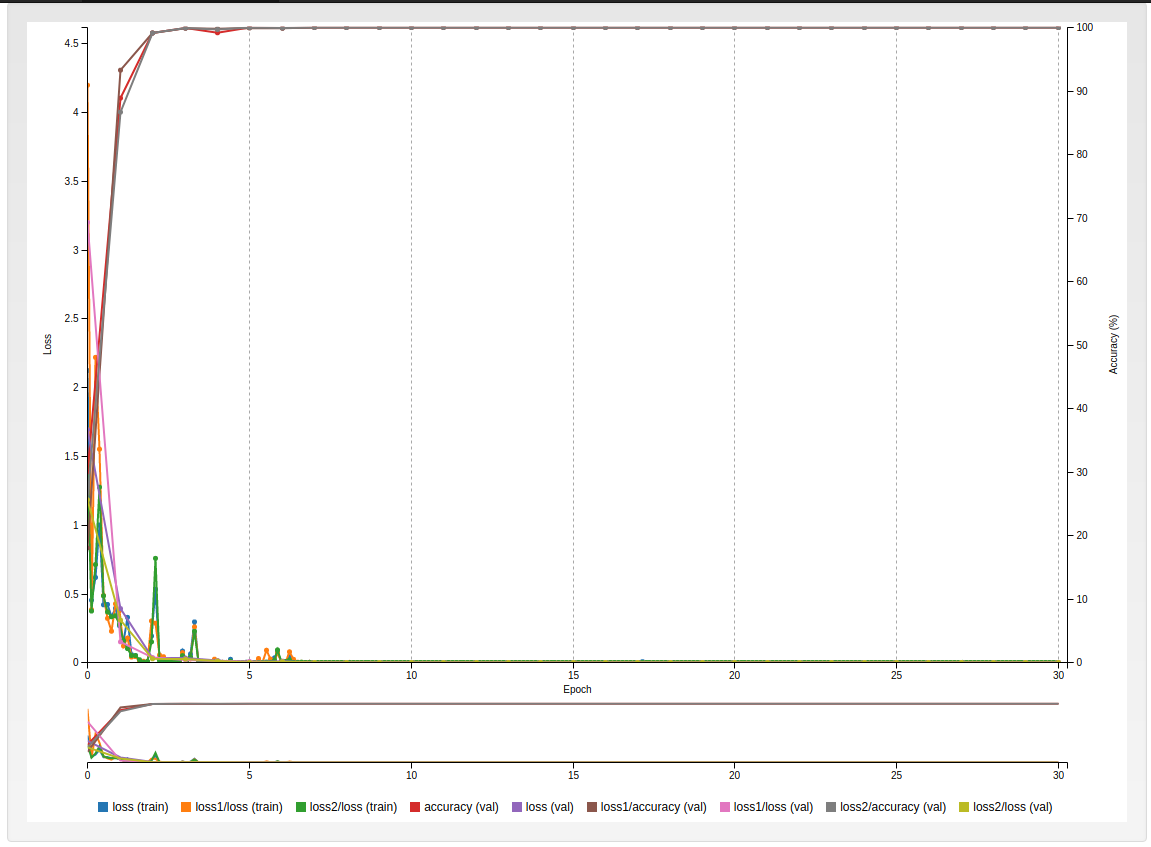
\includegraphics[width=\linewidth]{images/googlenet_training_loss.png}
      \caption{Training loss and accuracy variance curve on supplied data.}
      \label{fig:supplied-training-result}
\end{figure}



\subsection{On Collected Dataset}

GoogLeNet trained on the collected dataset converged at around 12th epochs. The training accuracy and validation accuracy were almost the same but only reached 73\%.

\begin{figure}[thpb]
      \centering
      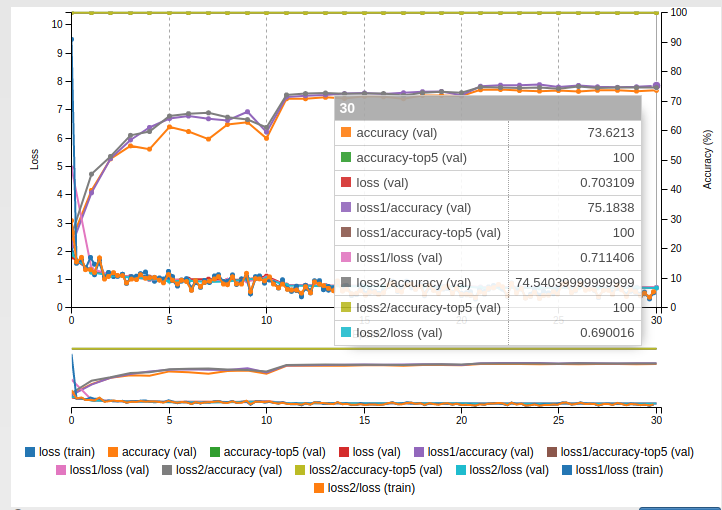
\includegraphics[width=\linewidth]{images/googlenet_flowers_training_loss.png}
      \caption{Training loss and accuracy variance curve on collected data.}
      \label{fig:collected-training-result}
\end{figure}

\section{Discussion}

The provided evaluate function could be used on the supplied dataset. After 30 epochs' training, the trained model could reach as high as 75.40\% test accuracy on an unseen test dataset. The inference time were a little higher than 5 ms which was within 10 ms which meets the requirement. Both results are shown in Fig. \ref{fig:supplied-evaluate}.

The test accuracy was much lower than the training accuracy which could happen for several reasons. Firstly, the dataset is small and the training is likely to overfit. The training accuracy is as high as around 100\% but it don't mean the similar performance when it comes to an unseen image. The issue could be addressed by data augmenting. Secondly, the model is over complicated for the data which also could lead to the overfit problem. One solution could be introducing more dropout layers. But in general, the performance is good enough for the robotic inference application.

\begin{figure}[thpb]
      \centering
      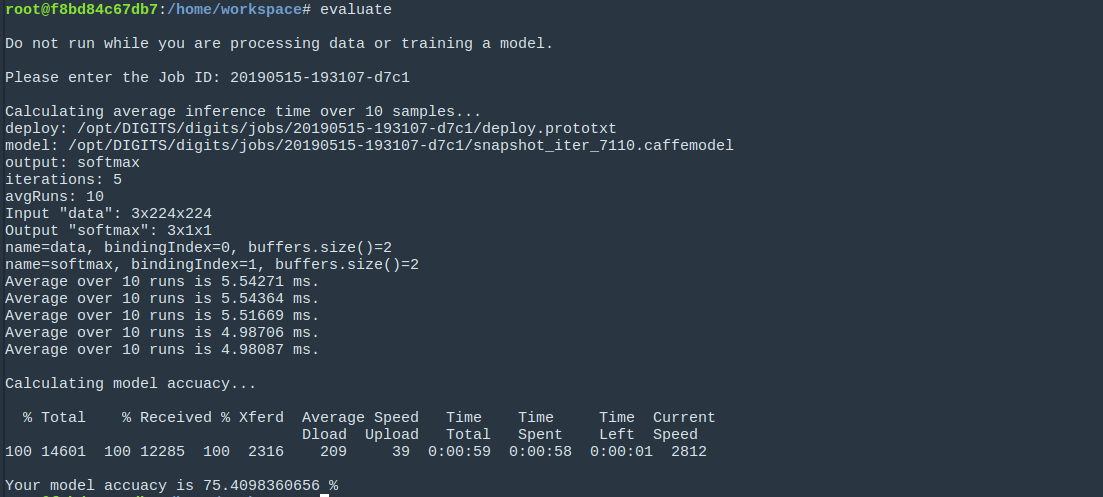
\includegraphics[width=\linewidth]{images/evaluate_screenshot.png}
      \caption{Model evaluation after training.}
      \label{fig:supplied-evaluate}
\end{figure}

\section{Future work}
In this project, Nvidia DIGITS as Deep Learning platform was used to train models for image classification tasks. Firstly, a supplied dataset with 3 classes was trained with a GoogLeNet network and achieved 75.41\% evaluation accuracy and under 10 ms inference speed. While with collected dataset, Flowers, the model trained based on GoogLeNet achieved 73\% training accuracy.

One direct improvement for training is to purify the collected data. The images were randomly captured from internet containing a piece of garbage data which might decrease the prediction or recognition level.

The test on the embeded hardware, namely Jetson TX1/TX2, is expected to be done when it is available. Then inference speed and real time recognition could be presented.

\bibliography{bib}
\bibliographystyle{ieeetr}

\end{document}